% !TEX program = lualatex
\documentclass[12pt]{article}

% Use fontspec to select fonts
\usepackage{fontspec}
\usepackage{amsmath}
\usepackage{amsfonts}
\usepackage{amsthm}
\usepackage{amssymb}
% \usepackage{unicode-math}
% \usepackage{polyglossia}
\usepackage{graphicx}
\usepackage{hyperref}
% \usepackage{bidi}


% Use polyglossia to set the document language
\usepackage{polyglossia}
\setmainlanguage{hebrew}
\setotherlanguage{english}
\renewcommand{\qed}{\hfill\blacksquare}
% Select a Hebrew font (replace 'David CLM' with any Hebrew font you have installed)
\newfontfamily\hebrewfont{David CLM}

% Use bidi for bidirectional text support, if needed. polyglossia may load this automatically.
% \usepackage{bidi}

% Additional packages for your document
\usepackage{graphicx}  % For including images
\usepackage{hyperref}  % For hyperlinks

% Document information
\title{הצעה לפיתרון מועד א' תשפד} % Your document's title

\begin{document}
\date{}
\maketitle
\begin{abstract}
    נא לקחת פיתרון זה בערבון מוגבל, במידה ואתם חושבים שמצאתם טעות בפיתרון נא לשלוח מייל למתן.
\end{abstract}

\section*{טענה 1}
$G\uparrow,T\uparrow$ ולכן בגלל השנ''צ $A_0\uparrow$. בעצם יש לנו הרחבה פיסקלית והזזה ימינה של $IS$:
\begin{enumerate}
    \item התוצר יגדל
    \item השינוי בתוצר יהיה בין 0-001
    \item החיסכון הפרטי יקטן
    \item השקעות ירדו
    \item החיסכון הציבורי לא ישתנה
\end{enumerate}
\section*{טענה 2}
כלכלן טוען: "אם הממשלה  תבצע צמצום פיסקלי כאשר התוצר שווה לתוצר הפוטנציאלי, יש חשש שגם ההשקעות ירדו." \\
הסבר : צמצום פיסקלי יגרום לירידה בתוצר דבר שעלול להקטין את הכנסות של העסקים ולכן יביא בירידה בהשקעות, בין אם זה אי היכולת של עסקים לממן את השקעות שלהם או סירוב של הבנקים לתת לבעלי העסקים הלוואות בגלל הכנסות נמוכות.
\section*{טענה 3}
\begin{equation*}
    \frac{K}{Y} = 2.5 \quad d = 4\% \quad S_L = 1-\alpha = 0.7 \quad  \widehat Y = 3\% = n+g
\end{equation*}
במהלך הקורס הראנו שבמצב יציב :
\begin{equation*}
    \frac{K}{Y} = \frac{s}{n+d+g} = 2.5 = \frac{s}{7\%} \implies s = 0.175 \neq \alpha = 0.3
\end{equation*}
משמע המשק לא באופטימום חברתי .\qed
\section*{טענה 4}
 פרטים בחלק התחתון של משקי הבית הם בעלי הכנסות נמוכות ובעלי צפי להכנסה נמוכה, לכן הם לא יכולים לקחת הלוואות ולמעשה תלויים אך ורק בהכנסה הנוכחית שלהם, בקורס קראנו לזה מגבלת נזילות. הכנסה שלהם מתואמת עם המחזור הכלכלי ובגלל שהם צורכים את כל הכנסתם, גם צריכתם תלוייה במחזור הכלכלי.
\section*{טענה 5}
שיעור הפחת ($d$) יורד ל4 אחוז והריבית עולה ל5 אחוז. לכן אין שינוי ברביע השני כי סכום של הפחת והריבית נשאר ללא שינוי אך כן יש שינוי ברביע הרביעי, פחות דירות נהרסות בכל תקופה ולכן מגיעים לש''מ חדש שבו יש יותר דירות. יש יותר דירות ולכן שכר הדירה יורד וגם מחיר הדירה.
\begin{equation*}
    d \downarrow \implies H^s \uparrow \implies R \downarrow \implies P_h \downarrow \qed
\end{equation*}

\section*{טענה 6}
\begin{equation*}
    \widehat Y = 6.5\% \quad \widehat K = 3\% \quad \widehat L = 4.5\% \quad S_K = \frac{1}{3} \quad S_L = \frac{2}{3}
\end{equation*}
\begin{enumerate}
    \item $$TFP = \widehat A = \widehat Y - \alpha \widehat K - (1-\alpha) \widehat L = \frac{1}{40} = 2.5\% $$
    \item נכון, ראינו בהרצאות ש $$MPL = \left(1-\alpha\right) y \implies \widehat{MPL}  = \widehat{y}= \widehat A + \widehat{k^\alpha} > \widehat A$$
\end{enumerate}
\section*{טענה 7}
הפרטים (הרציונלים) מבינים ומסתכלים על הצריכה הפרטית של הממשלה ולא על המיסים זאת משום שהם מבינים שאם הממשלה מורידה מיסים היום בלי להוריד צריכה ממשלתית היא נכנסת לגירעון וצריכה לקחת הלוואות, את הלוואות היא צריכה להחזיר בעתיד, ואיך היא תעשה זאת? על ידי העלת מיסים. לכן הפרטים בעצם חוסכים ליום שבו הממשלה תעלה בחזרה המיסים ולא משנים את צריכתם היום.

\newpage

\section*{מסה 1}
אנחנו יודעים את הדבר הבא:

\begin{equation}
    y_1 = 12 \quad  y_2 = 24
\end{equation}
\begin{equation}
    y_1 = 12 \quad  y_2 = 12
\end{equation}
\begin{equation}
    y_1 = x \quad  y_2 = 3x
\end{equation}

נתחיל מלפתור את הבעיה בכלליות
\begin{equation}
    C_1 + \frac{C_2}{1+r} = y_1 + \frac{y_2}{1+r}
    \label{Budget}
\end{equation}
זהו קו התקציב שלנו, בנוסף נתון לנו פונקציית התועלת של כל הפרטים
\begin{equation}
    U = \ln(C_1) + \ln(C_2)
    \label{Utility}
\end{equation}
$MRS$ הוא :
\begin{equation}
    MRS = \frac{C_2}{C_1} = 1+r \implies C_1 = \frac{C_2}{1+r}
    \label{MRS}
\end{equation}
נציב את משוואה \ref{MRS} במשוואה \ref{Budget} ונקבל:
\begin{equation}
    y_1 + \frac{y_2}{1+r} = 2C_1
\end{equation}
בעצם פה סיימנו את החלק הקשה בתרגיל, עכשיו פשוט "מנחשים" את הריביות והתחומים, נתחיל מפרט 1, ננחש שהוא לווה, נקבל ש:
\begin{equation}
    12 + \frac{24}{1+1.5} = 2C_1 \implies C_1 = 10.8 < y_1
\end{equation}
סתירה היות והנחו שהוא לווה, מכך אנחנו יכולים להסיק שהוא לא לווה.
נניח שהוא מלווה, נקבל:
\begin{equation}
    12 + \frac{24}{1+0.5} = 2C_1 \implies C_1 = 14 > y_1.
\end{equation}
שוב סתירה, מכך שהוא לא לווה ולא מלווה, כלומר לא משתתף בשוק ההון. \qed
\\ 
כעת נעבור לפרט 2, 
\begin{enumerate}
    \item נניח שהוא לווה, נקבל: \begin{equation}
        12 + \frac{12}{1+1.5} = 2C_1 \implies C_1 = 8.4 < y_1
    \end{equation}
    סתירה היות וקיבלנו שהצריכה שלו קטנה יותר מההכנסה שלו.
    \item נניח שהוא מלווה , נקבל : \begin{equation}
        12 + \frac{12}{1+0.5} = 2C_1 \implies C_1 = 10 < y_1
    \end{equation}
    אין סתירה לכן הוא מלווה. \qed
    
\end{enumerate}

כעת נעבור לפרט 3, נניח שהוא לווה, נקבל:
\begin{equation}
    x + \frac{3x}{1+1.5} = 2C_1 \implies C_1 = 1.1x > x
\end{equation}
אין סתירה, פרט 3 לווה. \qed
\newpage
\section*{מסה 2}
\begin{enumerate}
    \item הראשון טוען שהריבית תעלה והתוצר יגדל. \\
    הכלכלן הראשון ככל הנראה מניח הנחות קסיאניות רגילות, מורידים מיסים, ההכנסה הפנויה של הפרטים תעלה, הצריכה שלהם תגדל, מכך $IS$ זז ימינה, התוצר והריבית גדלים. \begin{equation*}
        T \downarrow \implies C \uparrow \implies Y \uparrow, r \uparrow
    \end{equation*}
    \item השני טוען שהריבית תעלה והתוצר יקטן, הוא מניח מודל צמיחה של סולו או בכללי מודל של ט''א, כאשר מורידים מיסים החיסכון קטן, מה שמקטין את מלאי ההון לעובד לאורך זמן  ומוריד את התוצר ומעלה ריבית,
    \begin{equation*}
        T \downarrow \implies s \downarrow \implies K \downarrow \implies Y \downarrow, MPK \uparrow \implies r \uparrow
    \end{equation*}
    \item השלישי הגיע למסקנה שהתוצר והריבית לא ישתנו, הוא מניח שקילות רקרדיאנית, הפרטים רואים שהמיסים יורדים אך הממשלה נכנסת לגירעון ולכת צריכה לקחת הלוואה, ובעתיד תצטרך לעלות מיסים כדי להחזיר את הלוואה, לכן הפרטים לא משנים את צריכתם ושום דבר לא משתנה.
\end{enumerate}
\newpage
\section*{מסה 3}
להלן נתונים של משק "עוץ" \footnote{קרדיט לעומר דגן על הפיתרון}
$$Y = K^{0.5}  \cdot \left(LE\right)^{0.5}$$
$$s=0.3 \quad d = 2\% \quad g = 2\%$$
$$K = 3,200 \quad L = 200 \quad E = 1$$

\begin{figure}[h]
    \begin{small}
        \begin{center}
            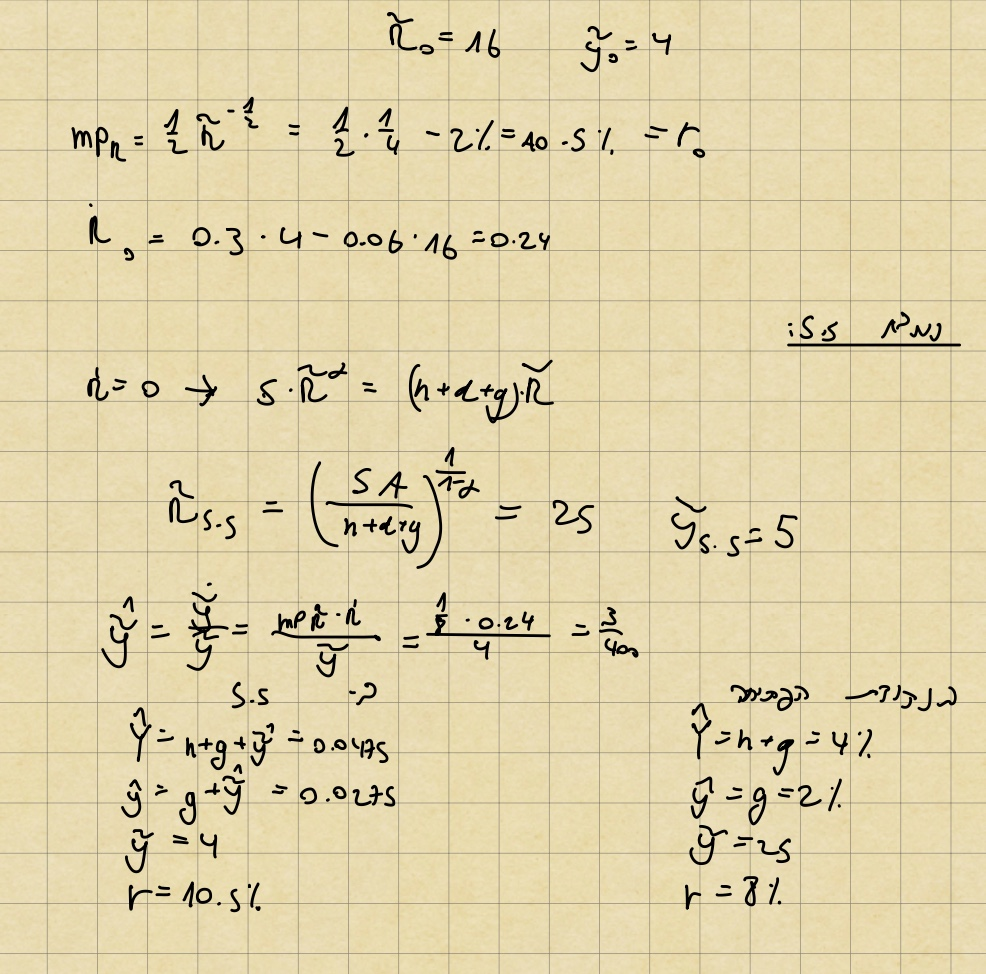
\includegraphics[width=0.85\textwidth]{figures/SCR-20240402-urdv.jpeg}
        \end{center}
    \end{small}
\end{figure}

\begin{figure}[h]
    \begin{small}
        \begin{center}
            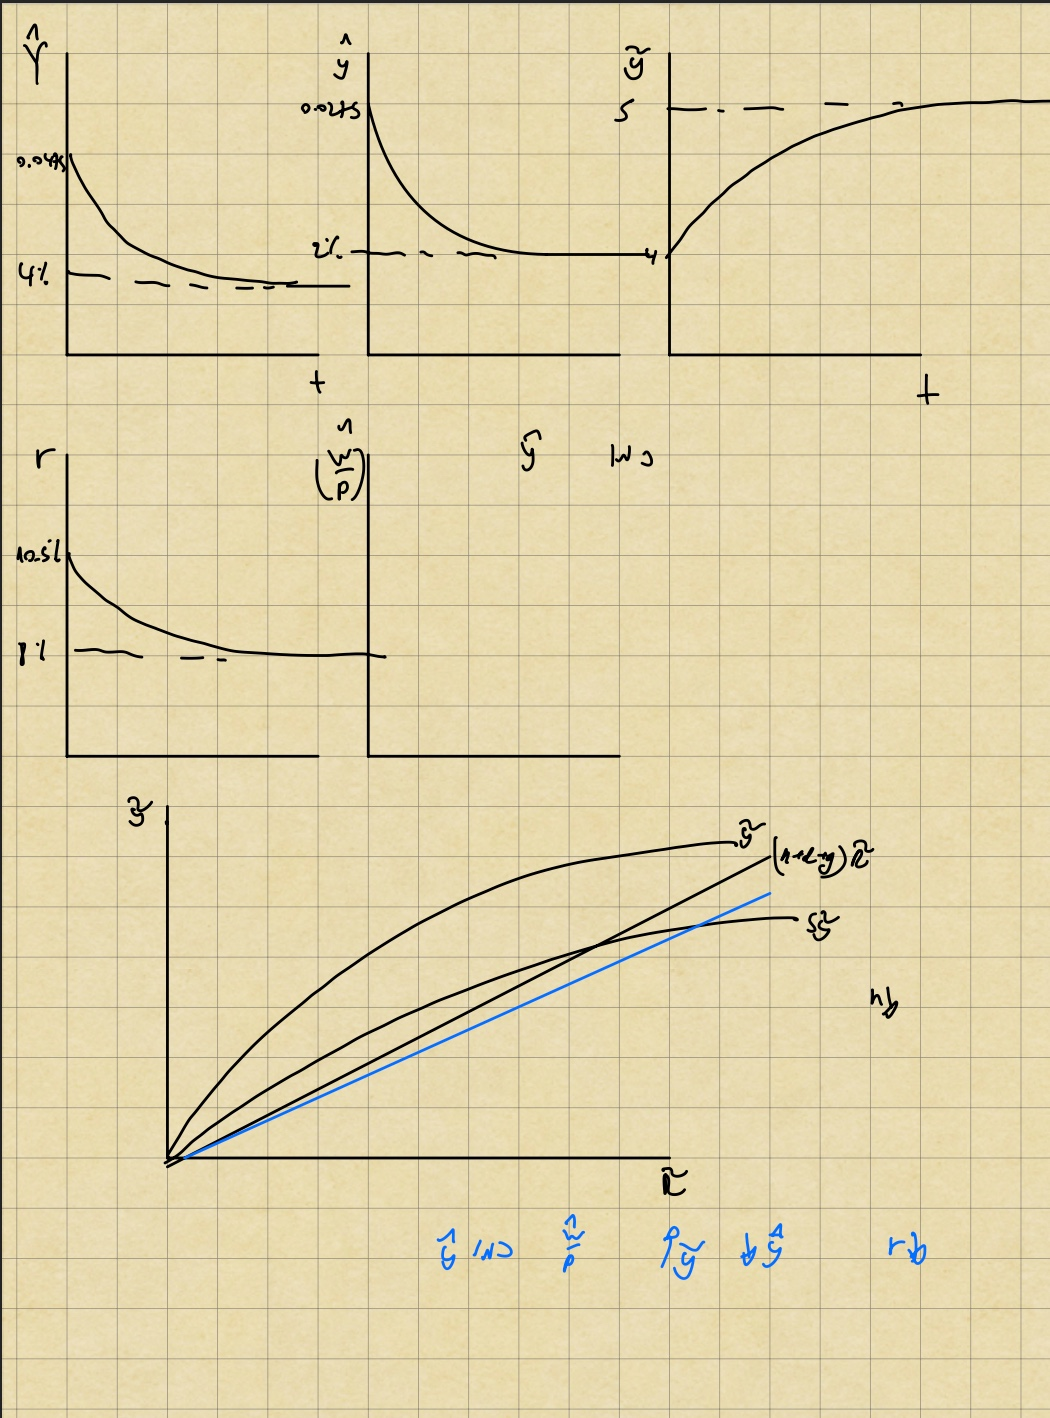
\includegraphics[width=0.85\textwidth]{figures/SCR-20240403-baer.jpeg}
        \end{center}
    \end{small}
\end{figure}



\end{document}